\subsection{Etude de l'user story}

	Le Fronting Digital est avant tout une application destiné aux banquiers afin de leur permettre de gérer plus efficacement et facilement leurs entrées en relation. Or, lors d'une ouverture de compte ou d'une souscription à une assurance vie il est obligatoire de fournir certains documents comme une pièce d'identité, un relevé d'identité bancaire ou encore un justificatif de domicile. Ici, ces documents sont appelés "pièces justificatives" et ont fait l'objet d'une user story sur laquelle j'ai travaillé de manière autonome, coinjointement avec un autre stagiaire. \\
	
	Le contenu de cette story concernait la mise en place d'un nouvel écran sur l'application depuis lequel il est possible d'uploader/downloader des pièces justificatives. Les pièces obligatoires qui doivent être fournies par le futur client de la banque dépendent de ses données personnelles. Par exemple, un client personne physique mineur ne fournira pas les même pièces qu'un client personne morale. Ainsi, le nouvel écran doit pré-afficher la liste des pièces obligatoires en la calculant au préalable à partir des données saisies par le banquier. La story mettait à notre disposition une matrice définissant l'ensemble des règles de gestion permettant de déterminer, à partir des données, si une pièce était obligatoire ou non. De plus, l'écran doit aussi proposer un menu déroulant permettant de choisir n'importe quel type de pièce afin de l'ajouter manuellement à la liste. Les pièces ajoutées de cette manière sont facultatives et doivent être affichées d'une couleur différente. Il est possible de retrouver en annexe \ref{d1} une maquette illustrant ce nouvel écran. \\

	Comme nous l'avons expliqué dans la partie \ref{deroulementSprint}, la première étape pour l'équipe de développement consiste à prendre connaissance de l'user story afin de la découper en tâches unitaires. Ici, nous avons fait le choix de créer 5 tâches qui sont les suivantes :
	
	\subsubsection{Composant pièce justificative}
	Le composant "pièce justificative" est un composant Angular représentant la brique qui contient tous les éléments et options d'une pièce justificative à savoir :
	\begin{itemize}
		\item Le fichier
		\item La date de fin de validité
		\item L'accord dérogatoire
		\item La date d'upload du fichier
		\item La possibilité de supprimer la pièce
		\item La possibilité de visualiser la pièce (ou la télécharger si elle ne peut être visualiser sur le navigateur)
	\end{itemize}
	Cette brique est représentée par un rectangle rouge sur l'annexe \ref{d1}
	
	\subsubsection{Composant écran pièce justificative}
	Ce composant est l'écran sur lequel sont affichées les pièces justificatives sous la forme d'une liste dont les éléments sont les composants décrits précédemment. Celui-ci pré-remplie la liste avec les pièces définies comme étant obligatoires. Ainsi, le banquier aura un rapide aperçu des pièces qu'il doit demander à son client et n'aura qu'à uploader les fichiers pour compléter la liste. De plus, un menu déroulant doit être présent, permettant de rajouter des pièces manuellement à la liste, dites facultatives qui apparaissent d'une couleur différente. En outre, le service d'appel front devra être créé afin de pouvoir communiquer avec l'API et consommer les web services. En outre, l'écran doit être accessible depuis la barre de navigation principale de l'application et un compteur indiquant le nombre de pièces obligatoires fournies/totales (par exemple 2/5) doit figurer au-dessus de la barre.
	
	\subsubsection{Référentiel}
	Dans notre application apparait un certain nombre de données métiers constantes comme la liste des pays pour un client, la liste des départements pour la France ou encore la liste des formes juridiques pour une entreprise. Pour toutes ces listes de données un endpoint est ajouté et un service appelé \textit{référentiel} est créé. Ainsi, il est possible de les obtenir de manière simple depuis le front en consommant le service adéquat. Si les métiers ont le besoin de modifier les valeurs, il suffit d'apporter une simple modification rapide et cela permet de garder un code structuré et clair. Dans notre cas, un référentiel devait être créé afin de référencer tous les types de pièces justificatives prises en charge par la banque (carte d'identité, justificatif de domicile, etc... pour un total de 41 différentes).	
	
	\subsubsection{Backend}
	Comme son nom l'indique, cette tâche consiste à développer les services backend destinés à alimenter notre frontend. Cela implique la création du contrôleur et de tous les endpoints, le service dédié ainsi que le modèle permettant de gérer les pièces justificatives. De plus, cela inclut le paramétrage pour la limite de taille des fichiers à uploader ainsi que la validation des données reçues.
	
	\subsubsection{Moteur de calcul}
	Nous avons dit plus haut que l'écran des pièces dévait pré-afficher la liste des pièces obligatoires. Or, le fait qu'une pièce soit obligatoire ou non dépend des données personnelles du client de la banque. Ainsi, le moteur de calcul doit prendre en compte l'ensemble des règles de gestion métiers ainsi que les données entrées jusqu'à présent par le banquier dans l'application afin de définir la liste des pièces obligatoires puis la transmettre au composant écran. \\
	
	Comme je l'ai dit plus haut, j'ai travaillé sur cette story avec un autre stagiaire. Ainsi, nous nous sommes séparé les tâches avant de commencer c'est pourquoi je me suis plutôt occupé de la partie backend et lui de la partie frontend. Ce découpage permettait d'avancer en parallèle sans problèmes. \\
	
\subsection{Sprint planning}
	Après avoir étudier l'user story et définie les différentes tâches à réaliser, une réunion de type sprint planning a eu lieu afin de définir la charge de travail pour effectuer chacune d'entre elles. Au cours de cette réunion nous avons voté et la charge a été réparti de la manière suivante :
	
\begin{table}[h!]
	\center
	\begin{tabular}{| c | c |}
     \hline
     Tâche & Charge (jour) \\ \hline
     Composant pièce justificative & ?\\ \hline
     Composant écran justificatifs & ?\\ \hline
     Backend & ?\\ \hline
     Référentiel & ?\\ \hline
     Moteur de calcul & ?\\
     \hline
	\end{tabular}
	\caption{Sprint planning pièces justificatives}
	\label{sprintPlanningPJ}
\end{table}

	Une fois le sprint planning terminé nous avons pu passer à la conception de nos tâches respectives ainsi qu'à la phase de développement.

\subsection{Conception}

	Dans un premier temps, j'ai commencé par définir les différents cas d'utilisation possible d'un banquier qui utiliserait l'écran des pièces justificatives. Il est possible d'observer ces cas sur le diagramme figure \ref{useCasePJ}.

\begin{figure}[h!]
	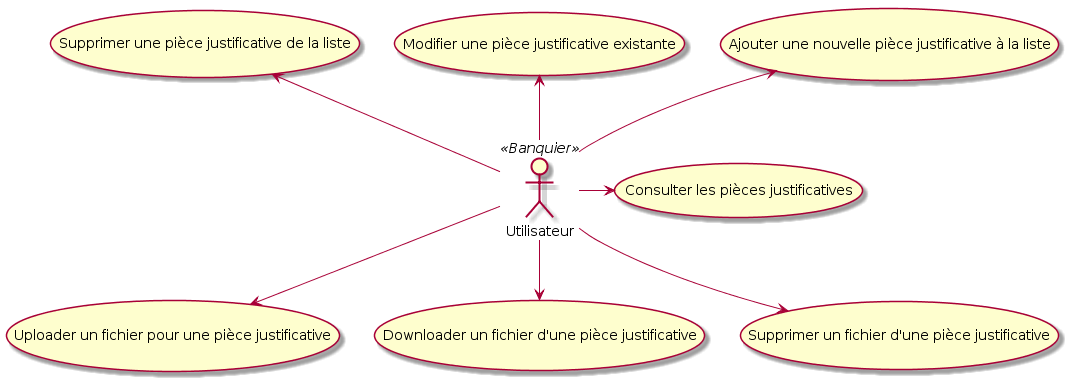
\includegraphics[scale=0.50]{images/travailBP1818/piecesJustif/useCasePJ.png}
	\centering
	\caption{Cas d'utilisation}
	\label{useCasePJ}
\end{figure}

	Une fois ces derniers définis j'ai pu procéder à la création du contrôleur ainsi que des endpoints permettant d'exposer les services répondant aux cas d'utilisation. Pour cela, il a fallu déterminer les méthodes HTTP et l'url associée que notre client pourra intéroger en essayant de rester RESTful. Le tableau suivant décrit les endpoints ainsi créés :
	
\begin{table}[h!]
	\center
	\begin{tabular}{| c | c |}
     \hline
     Méthode HTTP & URL \\ \hline
     GET & /justificatifs/{idForm}\\ \hline
     POST & /justificatifs/{idForm}/justificatif\\ \hline
     PUT & /justificatifs/{idForm}/justificatif\\ \hline
     DELETE & /justificatifs/{idForm}/justificatif\\ \hline
     GET & /{idForm}/fichier\\ \hline
     POST & /{idForm}/fichier\\ \hline
     DELETE & /{idForm}/fichier\\ \hline
	\end{tabular}
	\caption{Sprint planning pièces justificatives}
	\label{sprintPlanningPJ}
\end{table}

\begin{figure}[h!]
	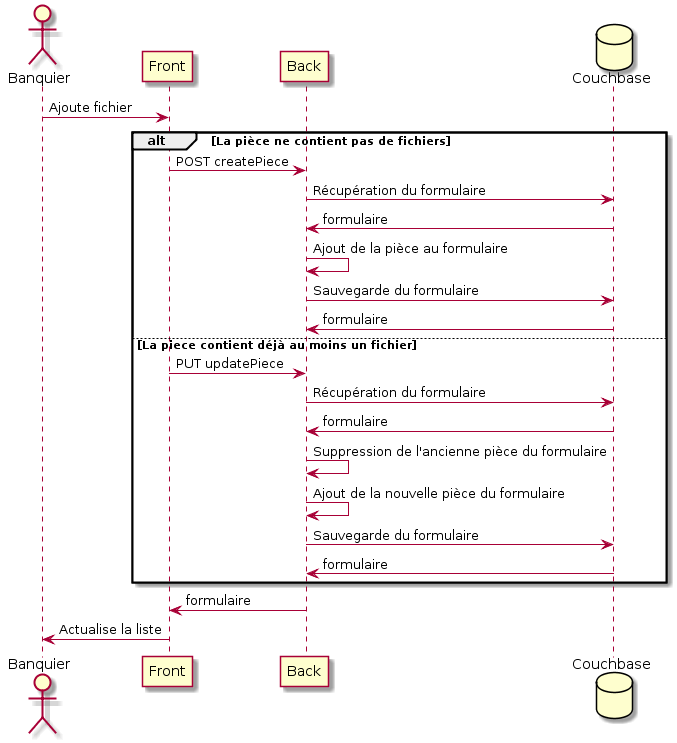
\includegraphics[scale=0.55]{images/travailBP1818/piecesJustif/seqSave.png}
	\centering
	\caption{Sauvegarde des pièces justificatives}
	\label{seqSave}
\end{figure}

\begin{figure}[h!]
	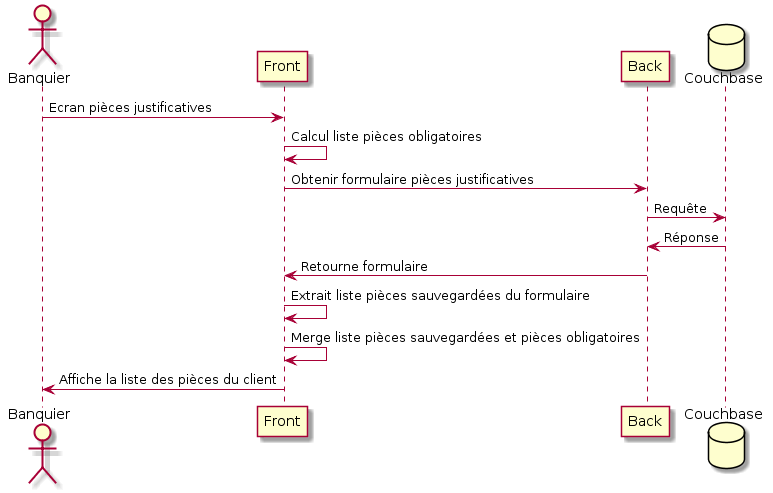
\includegraphics[scale=0.55]{images/travailBP1818/piecesJustif/seqGet.png}
	\centering
	\caption{Affichage des pièces justificatives}
	\label{seqGet}
\end{figure}

\subsection{Réalisation}

\subsection{Résultats et perspectives}
	
	
	\newpage
\begin{itemize}
	\item prendre connaissance user story + besoin client OK
	\item découpage en tâche sur github OK
	\item sprint planning (tableau avec les temps)
	\item définition du modèle
	\item définition des endpoints
	\item référentiel
	\item pb avec swagger
	\item moteur de scoring front (règles de gestion)
	\item TU
	\item resultat obtenu (retard tableau comparatif + pourquoi + mesure)
\end{itemize}